\documentclass[10pt]{article}

\usepackage{spheric}
%%%TITLE
\title{Numerical simulation of water-entry problems using an improved multiphase SPH method}
\date{}

%%AFFILIATIONS

\author[$\relax$]{H. Cheng}
\author[$\relax$]{A.M. Zhang}
\author[$\relax$]{F.R. Ming$^\dagger$}
\affil[$\relax$]{Harbin Engineering University, China}
\affil[$\relax$]{\email{\dagger}{mingfuren2006@126.com}}

%%DOCUMENT
\begin{document}

\maketitle

%\SelectedTopics{}

%%PLEASE PUT YOUR ABSTRACT HERE
\begin{abstract}
Water entry is a complex fluid-solid interaction problems that be focused in many aspects, i.e., the shipbuilding and aerospace. The impacting loads are hard to be predicted especially for the solid with a small deadrise angle, beacuse the effect of the air should be taken into account. In the paper, an improved multiphase SPH model is established to simulate the water entry of wedge with different deadrise angles. The Sub-Grid Scale (SGS) model with a multiphase form is adopted in the SPH scheme to represent the effect of the turbulence. What's more, the traditional shifting algorithm is improved for multiphase problems. Based on this, firstly, the water entry of the wedge and the plate are simulated and compared to the experimental data to validate the feasibility and accuracy of the SPH model in the paper. Then, the numerical simulations with variant deadrise angles are carried out, and the results are compared to the single-phase SPH model to investigate the effect of the air. 

The images of the water entry of wedge with deadrise angle of $30^\circ$ is presented in Figure \ref{fig:39}, where the wedge free falls from 1.93 m away from the water surface. The velocity field of the air and the pressure field of the fluid are represented respectively. At $t=0.62$ s, before the wedge contacts with water, the fluid pressure has been affected by the high-speed air flow around the wedge. The whole flow field during the impact is steady which verifies the viablility of the SPH model in the paper.

\begin{figure}[!htb]
\begin{minipage}[t]{0.33\linewidth}
\centering
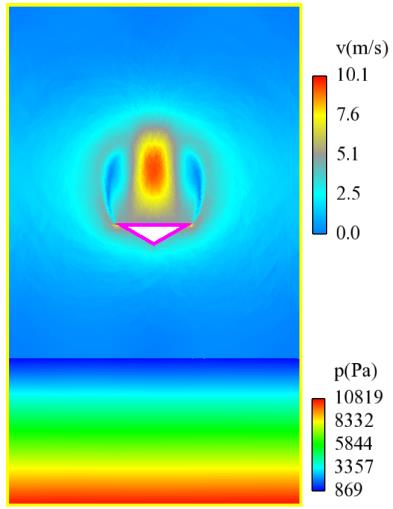
\includegraphics[width=0.8\textwidth]{39-11.png}\\
$t=0.30$ s
\end{minipage}
\begin{minipage}[t]{0.33\linewidth}
\centering
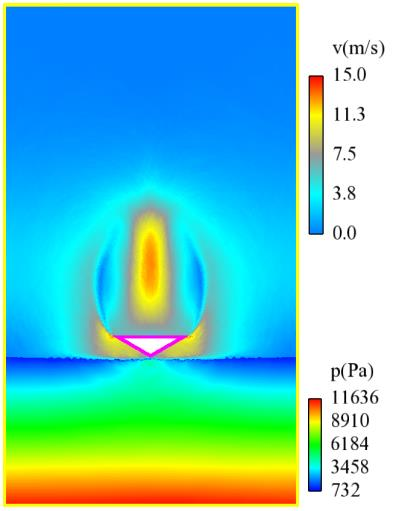
\includegraphics[width=0.8\textwidth]{39-12.png}\\
$t=0.62$ s
\end{minipage}
\begin{minipage}[t]{0.33\linewidth}
\centering
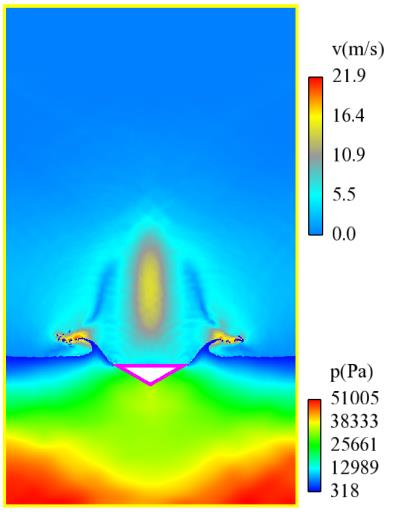
\includegraphics[width=0.8\textwidth]{39-13.png}\\
$t=0.65$ s
\end{minipage}
\caption{The images of water entry of wedge with deadrise angle of $30^\circ$.}\label{fig:39}
\end{figure}

\end{abstract}


%%THE END OF ABSTRACT

\addbib

\end{document}
